%% STORM-PhysNet -- IEEE CONFERENCE -- AGERS 2026 REVISED MANUSCRIPT (v2, corrected re-run)
%% All numbers come from report_final/ (combine_report.py over blocks A, B, C and GRASP folds G1-G3).
\documentclass[conference,a4paper]{IEEEtran}
\usepackage{amsmath,amssymb,amsfonts}
\usepackage{graphicx}
\usepackage{booktabs}
\usepackage{cite}
\usepackage{url}
\usepackage{placeins}

\title{STORM-PhysNet: A Multi-Horizon Transformer for Geostationary
Relativistic Electron Flux Forecasting and Cross-Satellite Transfer}

\author{
\IEEEauthorblockN{Samarth B N}
\IEEEauthorblockA{\textit{Dept.\ of Electronics and Communication Engineering} \\
\textit{RV College of Engineering}\\
Bangalore, India \\
samarthbn.ec25@rvce.edu.in}
\and
\IEEEauthorblockN{Samrudh S Malali}
\IEEEauthorblockA{\textit{Dept.\ of Electronics and Communication Engineering} \\
\textit{RV College of Engineering}\\
Bangalore, India \\
samrudhsmalali.ec25@rvce.edu.in}
\and
\IEEEauthorblockN{Dhyan M}
\IEEEauthorblockA{\textit{Dept.\ of Electronics and Communication Engineering} \\
\textit{RV College of Engineering}\\
Bangalore, India \\
dhyanm.ec25@rvce.edu.in}
\and
\IEEEauthorblockN{Sanjana H V}
\IEEEauthorblockA{\textit{Dept.\ of Artificial Intelligence and} \\
\textit{Machine Learning Engineering} \\
\textit{RV College of Engineering}\\
Bangalore, India \\
sanjanahv.ci25@rvce.edu.in}
}

\begin{document}
\maketitle

%% -----------------------------------------------------------------------
\begin{abstract}
Electrons above 2\,MeV at geostationary orbit (GEO) are a recurring
internal-charging hazard for communication, navigation and Earth-observation
satellites. We present STORM-PhysNet, a Transformer that forecasts GOES-15
\({>}2\)\,MeV log-flux 1, 6 and 12\,h ahead from a 72\,h history of flux and
OMNI solar-wind/geomagnetic drivers, with a learnable propagation delay,
a \(B_z\)-conditioned gate and residual-over-persistence heads. We evaluate it
under a leakage-free protocol (no back-filled gaps, causal Kp, boundary-buffered
windows) on three disjoint test periods (2012--13, 2015--16, 2018--20;
34\,554 windows, 937 storm-time windows, Dst down to \(-198\)\,nT), with ten
seeds per model and paired tests against an architecture-matched Transformer,
a residual-head Transformer, a flux-only Transformer and an LSTM.
STORM-PhysNet reaches a block-averaged prediction efficiency of
0.977/0.865/0.803 at 1/6/12\,h (persistence 0.968/0.581/0.261). It beats the
matched Transformer at 1\,h in every block (\(+0.008\), \(p=3.5\times10^{-18}\)),
ties it at 6\,h and trails it at 12\,h (\(-0.010\)). Ablations show that the
1\,h gain comes from the residual-over-persistence head and the 6--12\,h skill
from the solar-wind inputs; the delay and gate do not improve clean-data accuracy.
They do, however, coincide with much greater robustness: with unit-variance noise on
the drivers STORM-PhysNet keeps 1\,h PE at 0.970 (matched Transformer 0.892),
and on GSAT-19 GRASP data from an Indian-longitude GEO sensor it transfers
zero-shot with 12\,h PE 0.738 versus 0.644 (\(p=5.3\times10^{-4}\)).
After fine-tuning both models converge (0.802 vs 0.794).
\end{abstract}

\begin{IEEEkeywords}
Geostationary orbit, relativistic electrons, space weather, Transformer,
data leakage, transfer learning, prediction efficiency, GRASP
\end{IEEEkeywords}

%% ====================================================================
\section{Introduction}
%% ====================================================================
Relativistic electron fluxes (\(E>2\,\mathrm{MeV}\)) at GEO can rise by
several orders of magnitude within a day of a geomagnetic disturbance and
cause deep dielectric charging of spacecraft electronics~\cite{baker2018,horne2005}.
Operators of geostationary communication, navigation and Earth-observation
platforms therefore need forecasts at lead times of hours, and increasingly
at longitudes, such as the Indian sector, that GOES does not monitor.

Forecasting has progressed from linear prediction filters~\cite{baker1990}
and empirical models~\cite{perry2010} to neural
networks~\cite{wei2018,son2022} and, recently,
Transformers~\cite{tan2024,sun2024,sun2025}. Two issues limit how these
results can be compared and trusted. First, evaluation details matter as much
as architecture: interpolated or back-filled gaps, centred filters, interleaved
splits and single test years can all inflate skill~\cite{camporeale2019,kapoor2023},
yet few studies report seed variability or significance tests, and simple
baselines often rival Transformers~\cite{zeng2023,tan2024}. Second, models are
almost always trained and tested on one satellite, while new sensors such as
GRASP on GSAT-19 start with short records~\cite{zhao2025}.

This paper makes four contributions. (i) A leakage-free evaluation protocol
for hourly GEO flux forecasting with three disjoint test periods spanning the
ascending, declining and minimum phases of solar cycle~24, ten seeds per model
and paired statistics. (ii) STORM-PhysNet, a multi-horizon Transformer with a
learnable delay, a \(B_z\)-conditioned gate and residual-over-persistence heads,
together with controls that isolate each design choice. (iii) An attribution of
skill: residual heads explain the 1\,h gain, solar-wind drivers the 6--12\,h
skill, while the delay and gate do not raise clean-data accuracy but coincide
with markedly better robustness to corrupted drivers. (iv) A GOES-15\(\to\)GRASP
transfer study comparing zero-shot use, heads-only and full fine-tuning, and
training from scratch.

%% ====================================================================
\section{Related Work}
%% ====================================================================
\textit{Empirical and neural models.} Linear prediction filters relate GEO
electron flux to solar-wind speed~\cite{baker1990} and underlie NOAA's
operational REFM; comparing such models, Perry et al.~\cite{perry2010} found no
clear winner and a strong solar-cycle dependence of skill. Wei et al.~\cite{wei2018}
forecast daily \({>}2\)\,MeV flux one day ahead with an LSTM (PE 0.83--0.91 per
test year against 0.68 for persistence). Son et al.~\cite{son2022} forecast hourly
flux 1--72\,h ahead with a multilayer perceptron on 72\,h of solar-wind and index
inputs (PE 0.97 at 1\,h, 0.53 at 72\,h), using a split that interleaves months
of the same year. Forsyth et al.~\cite{forsyth2020} framed GOES-15 forecasting as
threshold exceedance and found persistence hard to beat at the lower threshold.

\textit{Transformers.} Tan et al.~\cite{tan2024} found a Transformer only slightly,
and not significantly, better than TPA-LSTM on GOES-15 flux. Sun et al.~\cite{sun2024}
compared LSTM and Transformer models on 5-min GOES-10 \({\geq}2\)\,MeV flux at
1--24\,h (test year 2005; persistence PE 0.913/0.572/0.207 and best Transformer
0.940/0.828/0.747 at 1/6/12\,h), with gaps linearly interpolated and inputs
selected on that year, and later improved daily fluence prediction with
pre-training and few-shot learning~\cite{sun2025}. None of these studies
reports multi-seed significance tests. In general time-series forecasting,
simple linear models can outperform Transformers~\cite{zeng2023}, and the
Temporal Fusion Transformer~\cite{lim2021} already combines gating with
multi-horizon outputs; our gate differs only in being conditioned on \(B_z\).

\textit{Evaluation and transfer.} Skill should be reported against persistence
as well as climatology~\cite{camporeale2019,morley2018}. Data leakage is a common
source of irreproducible ML results~\cite{kapoor2023}, and autocorrelated series
need temporally blocked validation~\cite{bergmeir2018}. Across satellites,
Zhao et al.~\cite{zhao2025} cross-calibrated FY-4A against GOES-15 and trained a
nowcasting model on the merged record, which outperformed one trained on GOES-15
alone. We are not aware of a study of fine-tuning regimes for GEO flux
forecasting on a new sensor such as GSAT-19 GRASP.

\begin{figure*}[!t]
\centering
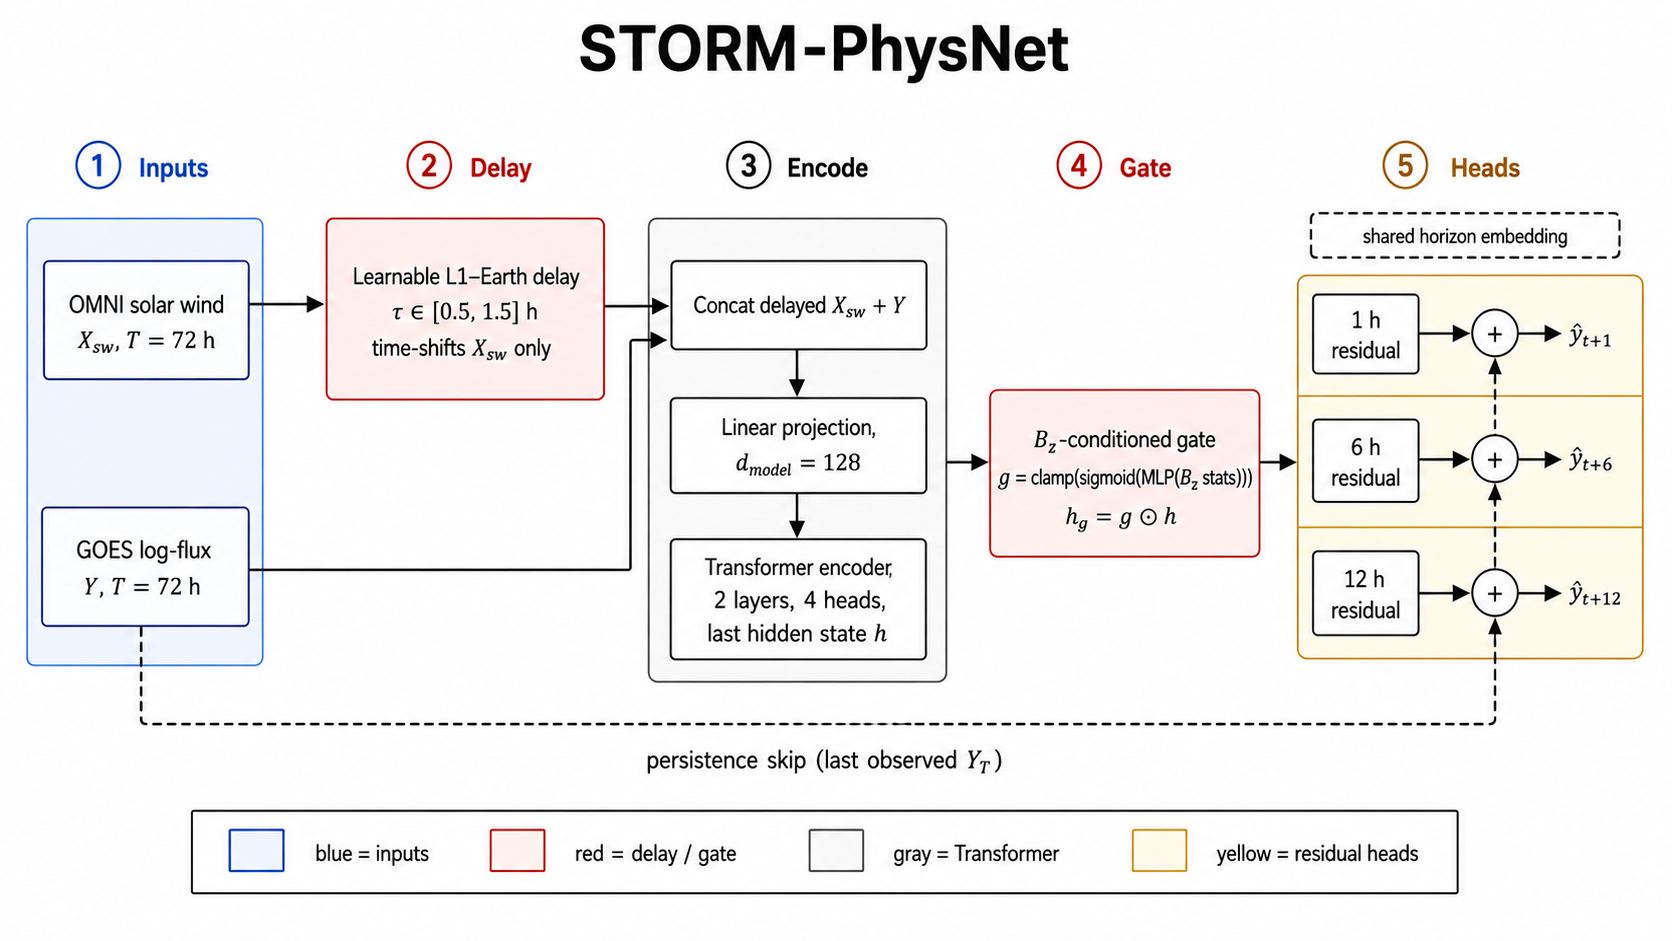
\includegraphics[width=0.80\textwidth]{figures/fig_system_architecture.png}
\caption{STORM-PhysNet. OMNI drivers are time-shifted by a learnable delay
\(\tau\in[0.5,1.5]\)\,h, concatenated with the GOES log-flux history
(\(T=72\)\,h), projected to \(d_{\mathrm{model}}=128\) and encoded by a
2-layer, 4-head Transformer. A \(B_z\)-conditioned gate scales the final
representation and three residual heads add corrections to persistence at
1, 6 and 12\,h.}
\label{fig:arch}
\end{figure*}

%% ====================================================================
\section{Data and Evaluation Protocol}
%% ====================================================================
\textbf{GOES-15 and OMNI.} The target is the GOES-15 EPEAD \({>}2\)\,MeV
integral electron flux from March 2010 to March 2020, averaged to hourly
means (87\,168 hours) and \(\log_{10}\)-transformed. Each forecast origin uses
72\,h of history of 18 channels: log-flux, its within-hour standard deviation,
an observed-flux mask, and 15 OMNI drivers and derived features (\(V_{sw}\),
\(B_z\), \(B_t\), density, \(P_{\mathrm{dyn}}\), duration of southward \(B_z\),
hours since storm onset, 1/6/24\,h means of \(V_{sw}\), 1/6\,h means of \(B_z\),
\(B_zV_{sw}\), Kp and Dst). OMNI is already propagated from L1 to the bow-shock
nose~\cite{king2005}.

\textbf{Leakage controls.} An audit of our earlier pipeline found four
leakage paths, each removed here. (1) Missing GOES hours (NOAA quality flags
or non-positive flux; 27--32\% of training hours) were back-filled from later
observations; now they are never filled: input histories are forward-filled
(past values only), the mask channel marks real hours, and a window is scored
only if its last input hour and all three target hours are observed. (2) A
centred Hampel despiking filter was removed. (3) OMNI repeats each 3-hourly Kp
value on all three hours, exposing up to 2\,h of future; each hour now sees only
the last completed Kp interval. (4) Each row is labelled
train/validation/test and a window is kept only if all 84 rows (72 input plus
12 lead) share one label, giving an 84\,h buffer at every boundary. Scalers are
fitted on training rows only.

\textbf{Blocked test periods.} The validation period (March 2017 to September
2018) is shared; three test blocks are evaluated separately, each model being
retrained with all remaining hours as training data (Table~\ref{tab:blocks}).
Blocks B and C contain the strong storms of 2015 and 2012--13. Because
training data then lie on both sides of the test block, this is blocked
cross-validation rather than strict forward chaining~\cite{bergmeir2018}.
Fig.~\ref{fig:blocks} shows the design.

\begin{figure}[!t]
\centering
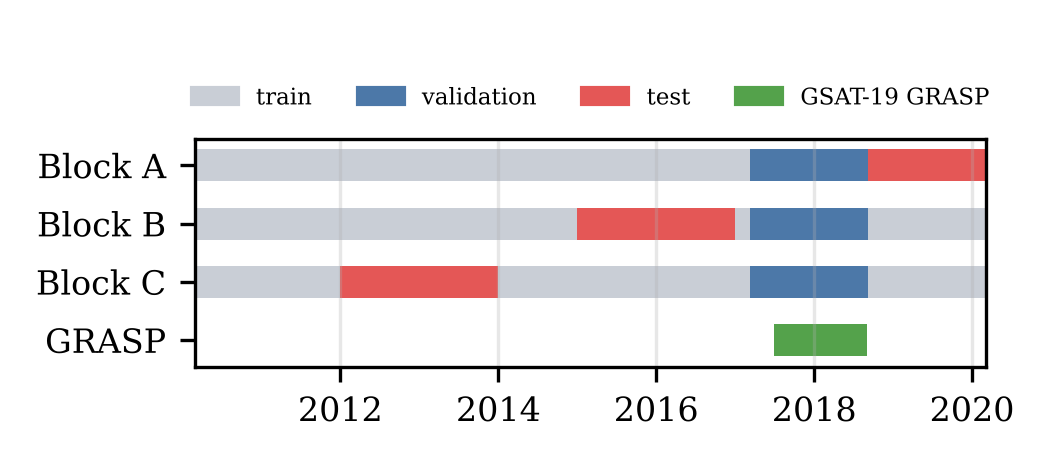
\includegraphics[width=\columnwidth]{figures/fig_blocks.png}
\caption{Evaluation design. Each GOES-15 block is a separate retraining with
its own test period and a shared validation period; GRASP (GSAT-19) data cover
July 2017 to August 2018.}
\label{fig:blocks}
\end{figure}

\begin{table}[!t]
\centering
\caption{Test blocks. Storm windows have Dst \(\le-50\)\,nT at the 6\,h target.}
\label{tab:blocks}
\setlength{\tabcolsep}{3pt}
\footnotesize
\begin{tabular}{lcccccc}
\toprule
Block & Test period & Train & Test & Gap-free & Storm & Min Dst \\
\midrule
A & 09/2018--03/2020 & 38\,909 & 7\,536 & 4\,283 & 18 & \(-69\) \\
B & 01/2015--12/2016 & 32\,296 & 14\,021 & 8\,452 & 565 & \(-198\) \\
C & 01/2012--12/2013 & 33\,413 & 12\,997 & 7\,189 & 354 & \(-139\) \\
\bottomrule
\end{tabular}

\vspace{0.5ex}
{\footnotesize \raggedright Window counts; validation has 9\,264 windows in
all blocks. Gap-free: no unobserved hour in the 72\,h input. Min Dst is over the 6\,h targets.\par}
\end{table}

\textbf{Metrics and statistics.} We report prediction efficiency against
climatology and persistence~\cite{morley2018},
\begin{align}
\mathrm{PE}_{\mathrm{clim}} &= 1 - \mathrm{MSE}(\hat y,y)/\mathrm{Var}(y), \\
\mathrm{PE}_{\mathrm{pers}} &= 1 - \mathrm{MSE}(\hat y,y)/\mathrm{MSE}(y_t,y),
\end{align}
where \(y_t\) is the last observed log-flux. PE without a subscript means
\(\mathrm{PE}_{\mathrm{clim}}\). Every model is trained with seeds 42--51 in
each block (210 GOES runs). Tables give seed means averaged over blocks;
comparisons use paired \(t\)-tests over the 30 seed--block pairs with
Cohen's \(d_z\), and bagged (seed-averaged) predictions get 95\% intervals
from a 7-day block bootstrap. P-values are not corrected for multiple comparisons.

\textbf{GRASP.} The Geostationary Radiation Spectrometer on GSAT-19
(\(\approx82^\circ\)E; data from ISSDC) provides \({>}2\)\,MeV electron flux from
July 2017 to August 2018 (10\,249 hours, 10\,158 observed; an hour needs at
least 6 of its 12 five-minute samples). GRASP is not cross-calibrated to
GOES, and we hold all driver channels at their GOES training mean, so the
experiment tests transfer of the flux-history model under sensor and longitude
shift. Three chronological folds use training from July 2017 up to the fold,
one month of validation and a 2--3-month test: G1 February--March 2018 (1\,316
test windows, no storm), G2 April--May 2018 (1\,381; 13 storm targets) and G3
June--August 2018 (2\,109; 47 storm targets from the 25--26 August storm).

%% ====================================================================
\section{Model and Baselines}
%% ====================================================================
\textbf{STORM-PhysNet} (Fig.~\ref{fig:arch}; 343\,599 parameters) has three
additions to a standard Transformer encoder~\cite{vaswani2017}
(\(d_{\mathrm{model}}=128\), 2 layers, 4 heads, \(d_{\mathrm{ff}}=256\)).
\emph{Adaptive delay:} a small network predicts a per-window shift
\(\tau\in[0.5,1.5]\)\,h applied to the driver channels by differentiable
interpolation, intended to absorb residual solar-wind timing error.
\emph{\(B_z\) gate:} an MLP of southward-\(B_z\) statistics produces a clamped
sigmoid vector \(\mathbf g\in[g_{\min},1]^{128}\) that scales the final encoder
state. \emph{Residual heads:} three heads with a shared horizon embedding
predict corrections to persistence, \(\hat y_{t+h}=y_t+\Delta_h\).
Training minimises a \(\beta\)-NLL loss~\cite{seitzer2022} on the three
horizons with a \(2.5\times\) penalty on storm-time under-prediction, plus small
auxiliary and regularisation terms (Dst/Kp, smoothness, monotonicity, delay and
coupling terms), using AdamW (learning rate \(3\times10^{-4}\)), cosine decay,
batch 64, storm windows oversampled \(12\times\), up to 40 epochs and early stopping on
the 12\,h validation MSE.

\textbf{Controls.} All controls use the same data, sampler and trainer.
\emph{Matched Transformer} (1.19\,M): STORM's \(d_{\mathrm{model}}\), depth and
heads with PyTorch's default \(d_{\mathrm{ff}}=2048\), no delay, gate or residual.
\emph{Transformer + residual head} (268\,k): \(d_{\mathrm{ff}}=256\) and the
persistence residual, but no delay or gate. \emph{Flux-only Transformer}: the
matched Transformer with all driver channels set to zero (flux history, its
within-hour spread and the mask kept). \emph{STORM ablations}:
no delay; no gate. \emph{LSTM} (55\,k). Compute was 23 T4 GPU-hours for the GOES runs.

%% ====================================================================
\section{Results}
\label{sec:results}
%% ====================================================================
\subsection{Skill on GOES-15}
Table~\ref{tab:main} and Fig.~\ref{fig:horizon} summarise test skill. All
learned models beat persistence clearly at 6 and 12\,h, where persistence
retains PE of only 0.581 and 0.261. At 1\,h persistence is already 0.968, and
only models with a persistence residual improve on it substantially
(\(\mathrm{PE}_{\mathrm{pers}}=0.25\)--0.32); the matched Transformer is level
with persistence (0.04) and the LSTM is worse (\(-0.97\)). The same pattern holds in each block (Fig.~\ref{fig:horizon}) and on gap-free
windows (STORM-PhysNet 0.980/0.857/0.798 in block A, for example).

\begin{table}[!t]
\centering
\caption{GOES-15 test skill, seed means averaged over blocks A--C.}
\label{tab:main}
\setlength{\tabcolsep}{2.4pt}
\footnotesize
\begin{tabular}{lccccccc}
\toprule
 & \multicolumn{3}{c}{\(\mathrm{PE}_{\mathrm{clim}}\), single model} & \(\mathrm{PE}_{\mathrm{pers}}\) & \multicolumn{3}{c}{\(\mathrm{PE}_{\mathrm{clim}}\), bagged} \\
\cmidrule(lr){2-4}\cmidrule(lr){6-8}
Model & 1\,h & 6\,h & 12\,h & 1\,h & 1\,h & 6\,h & 12\,h \\
\midrule
Persistence        & 0.968 & 0.581 & 0.261 & 0.00 & --- & --- & --- \\
LSTM               & 0.937 & 0.838 & 0.792 & \(-0.97\) & 0.946 & 0.860 & 0.815 \\
TF matched         & 0.969 & 0.867 & 0.813 & 0.04 & 0.975 & 0.884 & 0.833 \\
TF + residual      & 0.976 & \textbf{0.872} & \textbf{0.815} & 0.25 & 0.979 & \textbf{0.888} & \textbf{0.836} \\
TF flux-only       & 0.968 & 0.834 & 0.753 & 0.01 & 0.975 & 0.855 & 0.779 \\
STORM-PhysNet      & 0.977 & 0.865 & 0.803 & 0.29 & 0.979 & 0.881 & 0.825 \\
\quad no delay     & \textbf{0.978} & 0.869 & 0.806 & \textbf{0.32} & \textbf{0.980} & 0.883 & 0.827 \\
\quad no gate      & 0.977 & 0.867 & 0.805 & 0.28 & 0.978 & 0.882 & 0.828 \\
\bottomrule
\end{tabular}

\vspace{0.5ex}
{\footnotesize \raggedright Seed standard deviations are \(\le0.008\) for
STORM-PhysNet and the matched and residual Transformers. Bagged: the ten seed predictions are averaged before
scoring. Bold: best per column.\par}
\end{table}

\begin{figure*}[!t]
\centering
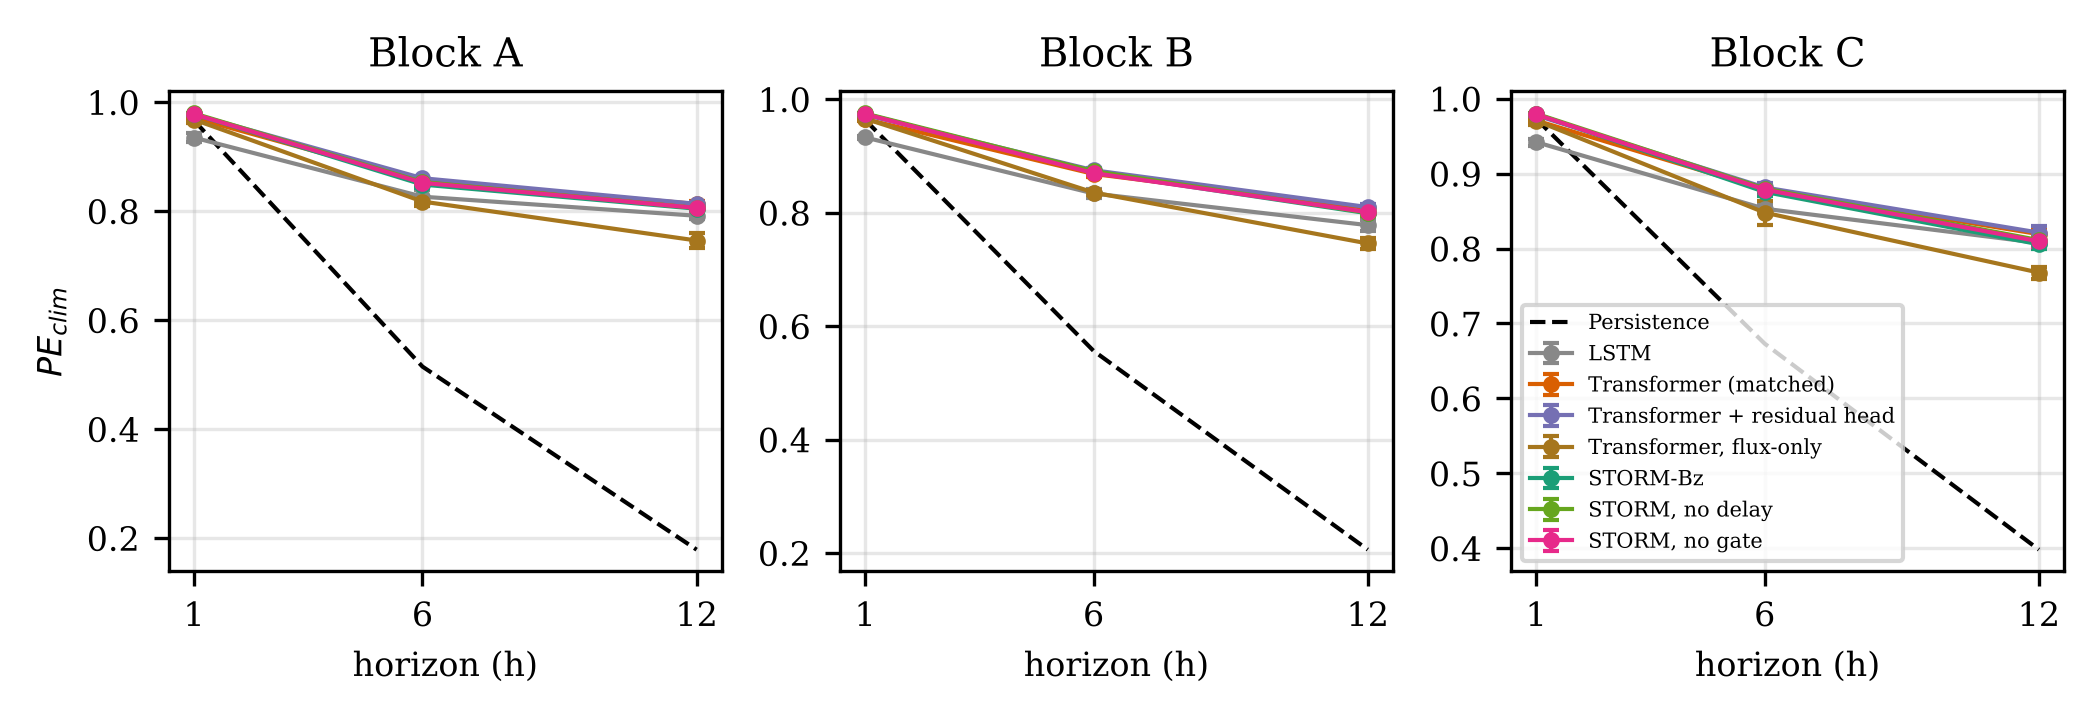
\includegraphics[width=0.86\textwidth]{figures/fig_horizon.png}
\caption{Test \(\mathrm{PE}_{\mathrm{clim}}\) against horizon in each block
(mean \(\pm\) standard deviation over ten seeds). Dashed: persistence. The
learned models are separated mainly from persistence and, at 6--12\,h, from the
flux-only Transformer.}
\label{fig:horizon}
\end{figure*}

\subsection{What Drives the Skill}
Table~\ref{tab:paired} gives paired differences. \emph{Against the matched
Transformer}, STORM-PhysNet is better at 1\,h in every block
(\(+0.0067\), \(+0.0091\), \(+0.0085\) in A, B, C), statistically tied at 6\,h
and worse at 12\,h in every block (\(-0.009\) to \(-0.014\)). The bootstrap
intervals of the bagged models agree: the 1\,h gain excludes zero in all
blocks, the 12\,h deficit in B and C.

\emph{Residual heads explain the 1\,h gain.} Adding only a persistence residual
to a plain Transformer raises 1\,h PE by 0.0069 (\(p=3.8\times10^{-17}\)) and
gives most of STORM-PhysNet's advantage; this smaller control is also the best
model at 6 and 12\,h. \emph{Solar-wind drivers explain the 6--12\,h skill:}
removing them leaves 1\,h PE unchanged (\(p=0.45\)) but costs 0.034 and 0.060 at
6 and 12\,h. \emph{The delay and gate do not improve clean-data accuracy:}
removing the delay slightly increases PE at all horizons, and removing the
gate changes nothing significantly. Fig.~\ref{fig:attr} shows that these
effects have the same sign in every block.

\begin{figure*}[!t]
\centering
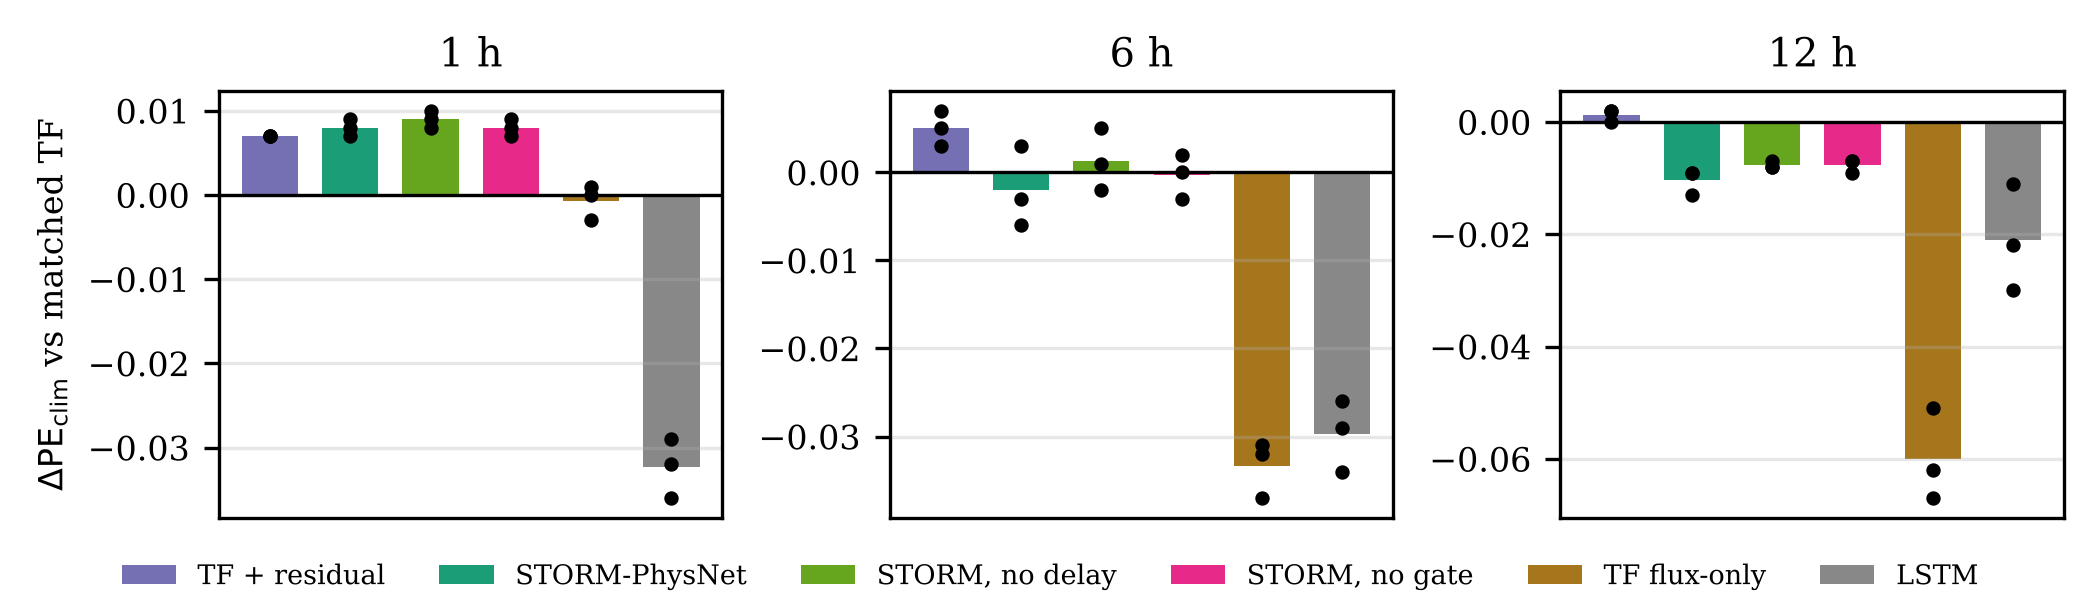
\includegraphics[width=0.86\textwidth]{figures/fig_attribution.png}
\caption{Difference in \(\mathrm{PE}_{\mathrm{clim}}\) from the matched
Transformer (bars: mean over blocks; dots: blocks A, B, C; each a ten-seed
mean). The persistence residual drives the 1\,h gain, the solar-wind inputs the
6--12\,h skill; the delay and gate add little.}
\label{fig:attr}
\end{figure*}

\begin{table}[!t]
\centering
\caption{Paired differences in \(\mathrm{PE}_{\mathrm{clim}}\) (30 seed--block pairs); \(p\)-values in parentheses.}
\label{tab:paired}
\setlength{\tabcolsep}{2.2pt}
\resizebox{\columnwidth}{!}{%
\begin{tabular}{lccc}
\toprule
Comparison & 1\,h & 6\,h & 12\,h \\
\midrule
STORM \(-\) TF matched & \(+0.0081\) (4e-18) & \(-0.0022\) (0.14) & \(-0.0104\) (1e-8) \\
STORM \(-\) TF + residual & \(+0.0012\) (5e-6) & \(-0.0071\) (9e-7) & \(-0.0118\) (4e-8) \\
TF + residual \(-\) TF matched & \(+0.0069\) (4e-17) & \(+0.0049\) (1e-3) & \(+0.0014\) (0.39) \\
TF matched \(-\) flux-only & \(+0.0008\) (0.45) & \(+0.0336\) (5e-17) & \(+0.0602\) (1e-20) \\
STORM \(-\) no delay & \(-0.0010\) (3e-8) & \(-0.0037\) (4e-5) & \(-0.0026\) (0.02) \\
STORM \(-\) no gate & \(+0.0002\) (0.11) & \(-0.0017\) (0.18) & \(-0.0024\) (0.05) \\
STORM \(-\) LSTM & \(+0.0406\) (1e-25) & \(+0.0273\) (9e-12) & \(+0.0107\) (3e-4) \\
\bottomrule
\end{tabular}}
\end{table}

\subsection{Storm Time and Events}
\begin{table}[!t]
\centering
\caption{RMSE of log-flux pooled over blocks A--C (seed means).}
\label{tab:storm}
\setlength{\tabcolsep}{3pt}
\footnotesize
\begin{tabular}{lcccccc}
\toprule
 & \multicolumn{3}{c}{Storm (937 windows)} & \multicolumn{3}{c}{Non-storm (33\,617)} \\
\cmidrule(lr){2-4}\cmidrule(lr){5-7}
Model & 1\,h & 6\,h & 12\,h & 1\,h & 6\,h & 12\,h \\
\midrule
Persistence    & 0.301 & 0.773 & 0.984 & 0.142 & 0.514 & 0.701 \\
LSTM           & 0.363 & 0.597 & 0.668 & 0.183 & 0.290 & 0.345 \\
TF matched     & 0.318 & 0.553 & 0.613 & 0.124 & 0.263 & 0.329 \\
TF + residual  & 0.292 & \textbf{0.548} & \textbf{0.606} & 0.113 & \textbf{0.258} & \textbf{0.327} \\
STORM-PhysNet  & \textbf{0.281} & 0.555 & 0.650 & 0.114 & 0.267 & 0.336 \\
\quad no delay & \textbf{0.279}\rlap{\(^*\)} & 0.554 & 0.642 & \textbf{0.111} & 0.264 & 0.335 \\
\bottomrule
\end{tabular}

\vspace{0.5ex}
{\footnotesize \raggedright Storm: Dst \(\le-50\)\,nT at the 6\,h target.
Bold: lowest error per column (\(^*\)ablation, not the proposed model).\par}
\end{table}

Table~\ref{tab:storm} splits the error into the 937 storm-time windows and
the rest. During storms STORM-PhysNet (with its no-delay ablation) has the
lowest 1\,h error, while at 6--12\,h all Transformer variants cut the
persistence error by 28--38\% and the residual Transformer is lowest; at 12\,h
STORM-PhysNet trails both Transformer controls. For
exceedance of \(10^{3}\)\,cm\(^{-2}\)s\(^{-1}\)sr\(^{-1}\), its 1\,h Heidke skill
score is 0.925--0.951 across blocks against 0.899--0.928 for persistence, and
at 12\,h it is 0.757--0.776 against 0.774--0.792 for the matched Transformer.
Fig.~\ref{fig:case} shows the June 2015 storm: after the dropout, the bagged
STORM-PhysNet follows the 24 June enhancement more closely than the matched
Transformer, but both miss the peak; this single event is illustrative only.

\begin{figure}[!t]
\centering
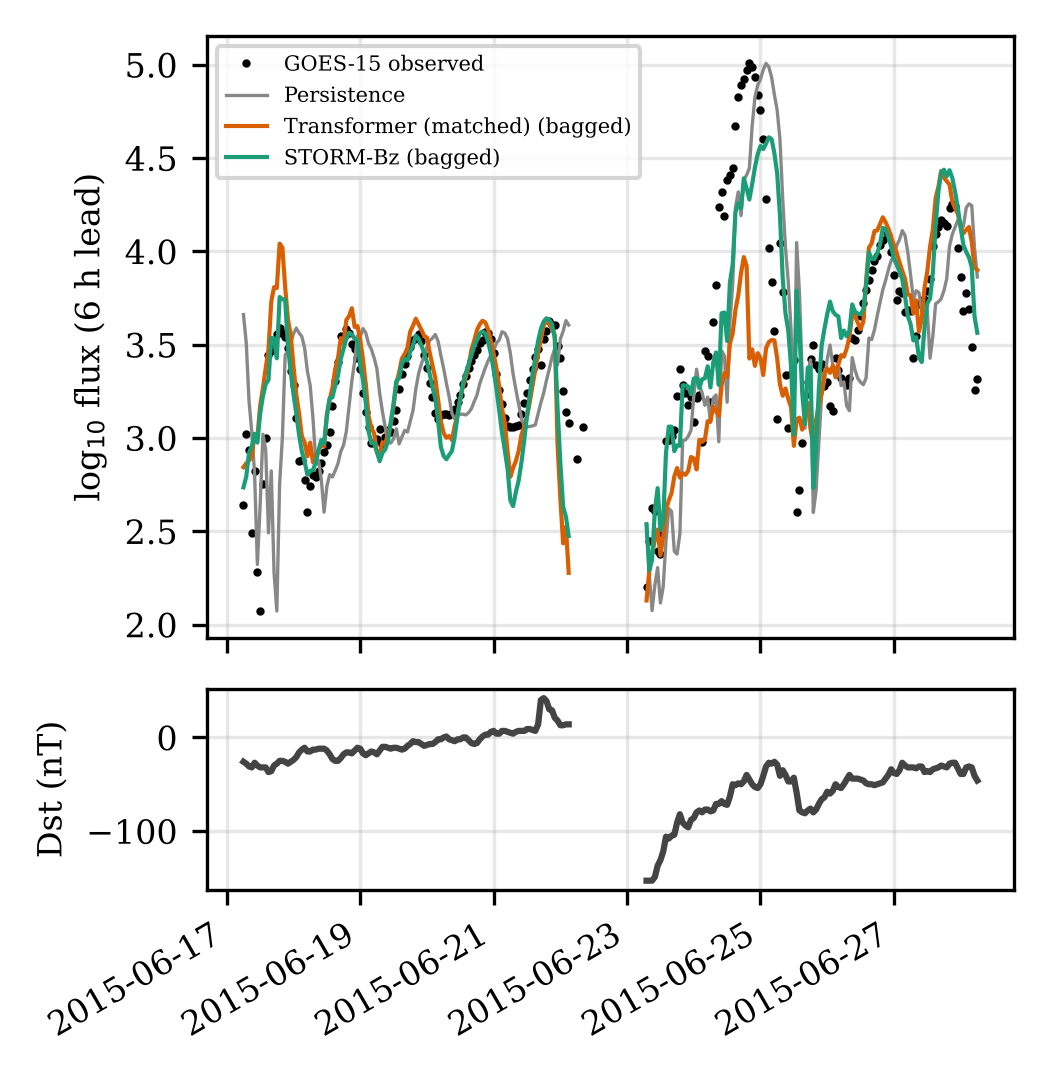
\includegraphics[width=0.82\columnwidth]{figures/fig_case_study.png}
\caption{6\,h forecasts (bagged over ten seeds) during the June 2015 storm,
block B. Gaps are unobserved hours; lower panel: Dst.}
\label{fig:case}
\end{figure}

\subsection{Robustness to Corrupted Drivers}
We add Gaussian noise of standard deviation \(\sigma\) (in standardised units)
to all driver channels of the test inputs, leaving the flux history unchanged
(Fig.~\ref{fig:noise}). At 1\,h STORM-PhysNet keeps PE at 0.970 for \(\sigma=1\)
and 0.960 for \(\sigma=2\), against 0.949 and 0.895 for the residual Transformer
and 0.892 and 0.651 for the matched Transformer. At 6\,h and \(\sigma=2\) the
values are 0.637, 0.554 and 0.481. Since the residual Transformer degrades
faster despite the same persistence anchor, this robustness is the one
measurable benefit associated with the delay and gate, possibly because the
gate limits how strongly the drivers can perturb the forecast; we did not run the ablations under noise,
so the two modules cannot be separated here.

\begin{figure*}[!t]
\centering
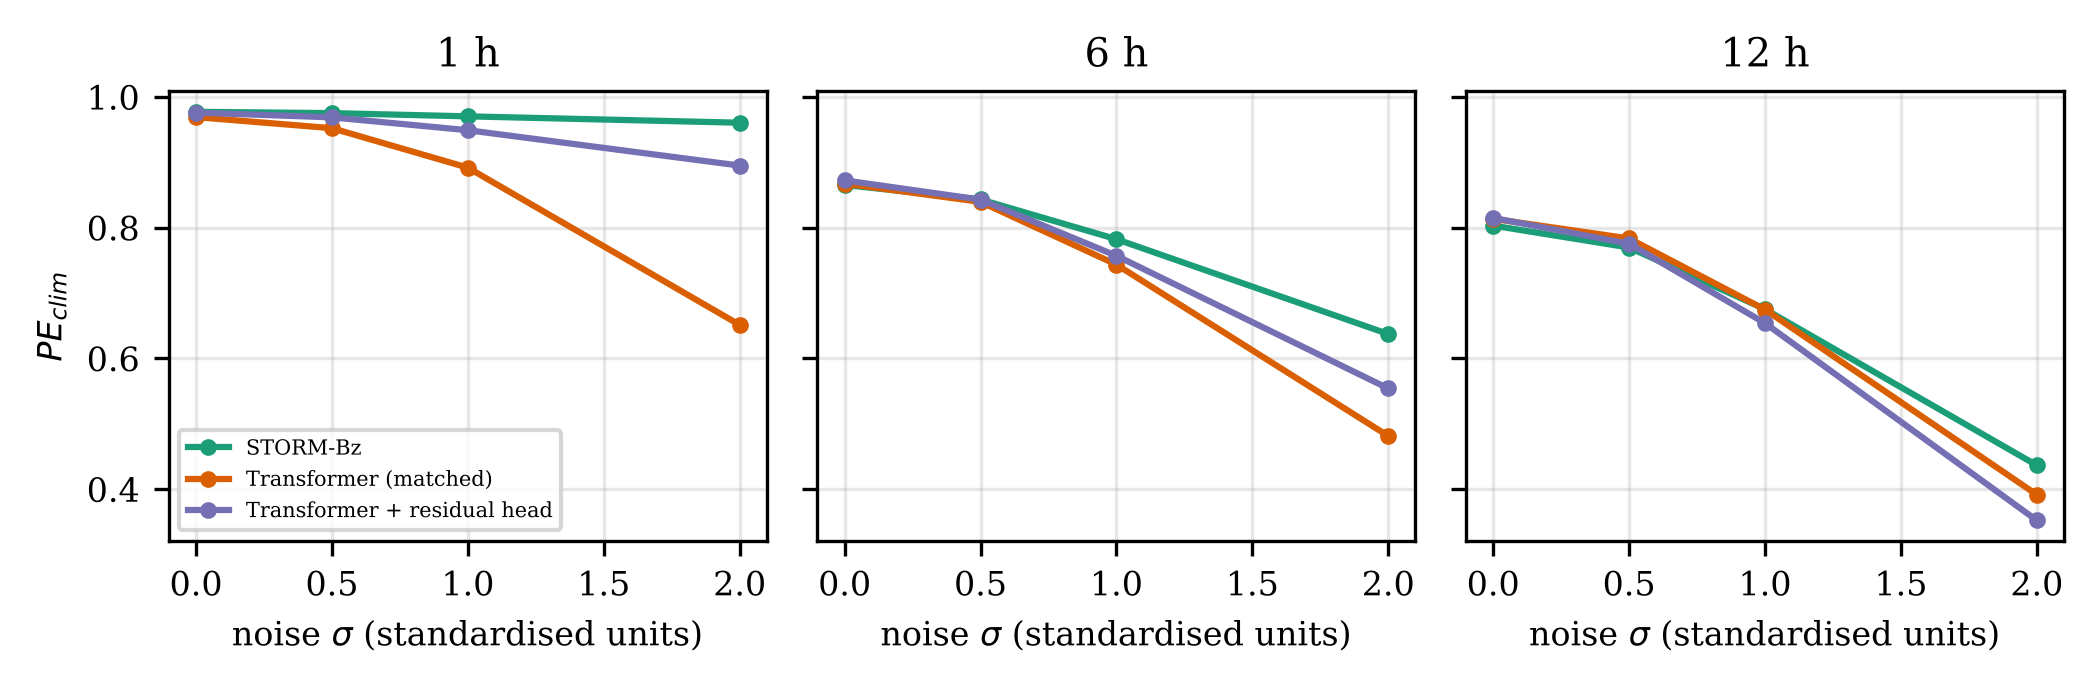
\includegraphics[width=0.78\textwidth]{figures/fig_noise.png}
\caption{\(\mathrm{PE}_{\mathrm{clim}}\) under Gaussian noise added to the
standardised driver channels (seed means averaged over blocks).}
\label{fig:noise}
\end{figure*}

\subsection{Interpretability}
The learned delay saturates: its mean is 1.50\,h and 92\% of test windows
(89--97\% per block) have \(\tau\ge1.49\)\,h, so the module acts as a constant
extra shift at the upper bound rather than a recovered transit time; because
OMNI is already propagated to the bow shock~\cite{king2005}, the preference for
older driver values is plausibly related to the hours-long acceleration
timescale~\cite{horne2005}. Gate activations are higher in storm than in quiet
windows (means 0.441 vs 0.424; area under the ROC curve
\(0.76\pm0.10\) over the 30 runs), so the gate responds to storm conditions,
but the shift is small (Fig.~\ref{fig:gate}).

\begin{figure}[!t]
\centering
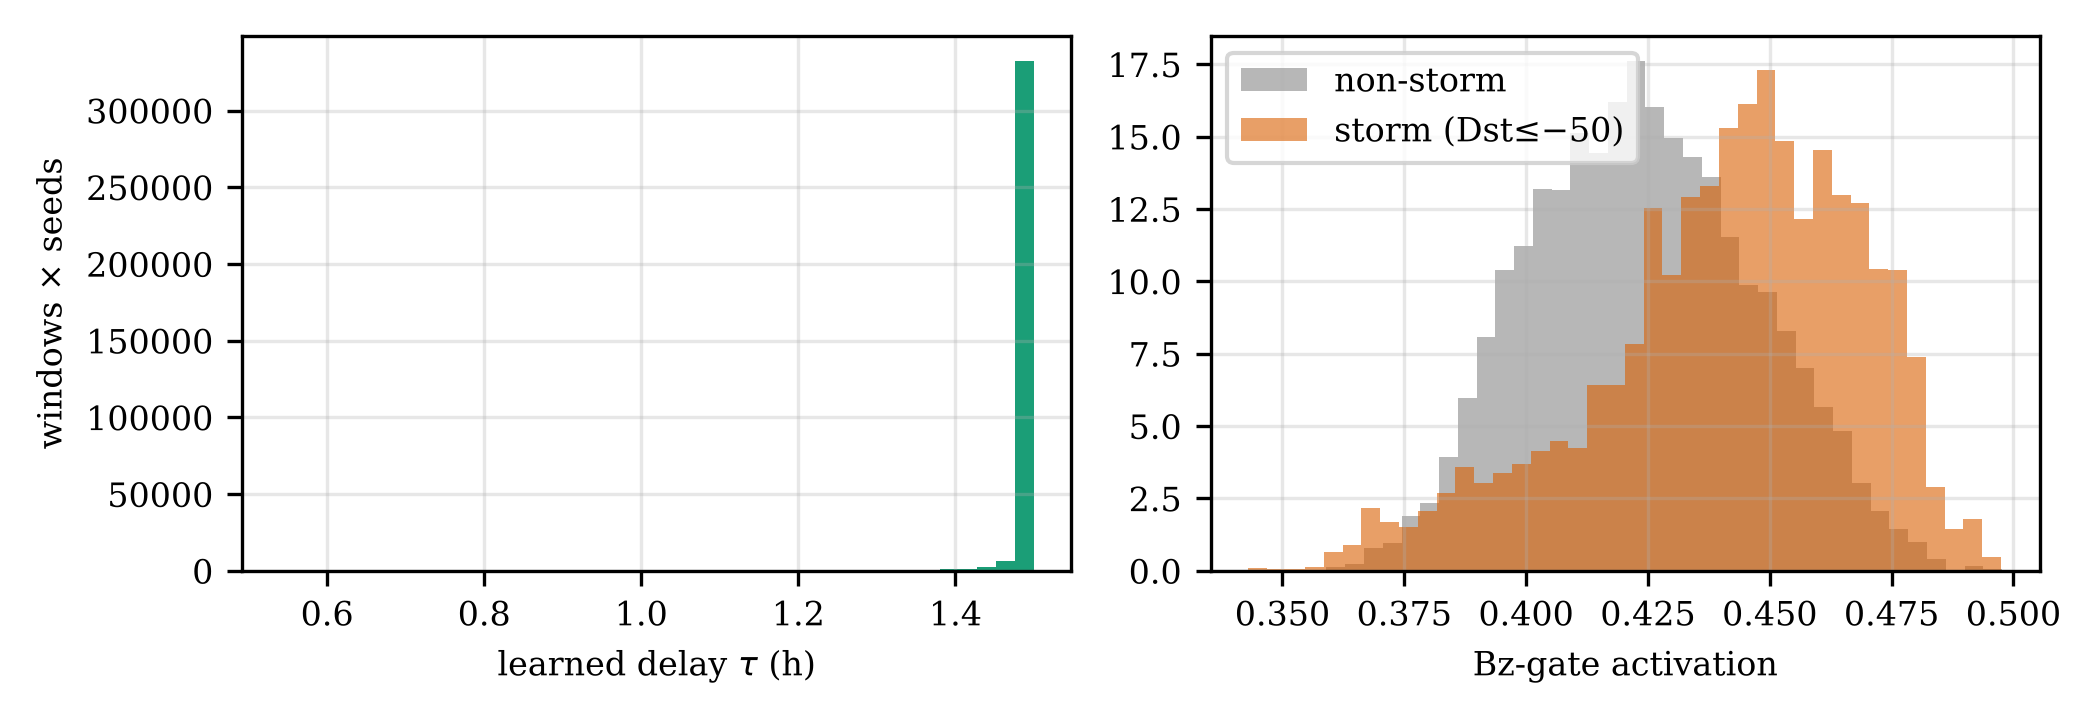
\includegraphics[width=\columnwidth]{figures/fig_gate_delay.png}
\caption{Left: learned delay over all test windows and seeds, piled at the
1.5\,h bound. Right: gate activation in storm and quiet windows (normalised
histograms).}
\label{fig:gate}
\end{figure}

\subsection{Transfer to GSAT-19 GRASP}
Table~\ref{tab:grasp} and Fig.~\ref{fig:grasp} compare four regimes, starting
from the block-A GOES models (persistence on GRASP: 0.951/0.529/0.129). Applied
zero-shot, STORM-PhysNet loses little at 1\,h and stays far above the matched
Transformer at all horizons (\(+0.075\), \(+0.075\), \(+0.095\);
\(p=6\times10^{-8}\), \(2\times10^{-5}\), \(5\times10^{-4}\)); the matched
Transformer falls below persistence at 1\,h. Fine-tuning the heads alone
recovers most of the gap (STORM-PhysNet 12\,h PE \(+0.049\),
\(p=8\times10^{-6}\)); this comparison is not like-for-like because STORM's
heads-only stage trains 63\,357 weights against 387 for the Transformer. With full
fine-tuning both reach the same skill (differences \(\le0.008\),
\(p\ge0.09\)), and training on GRASP alone is as good as fine-tuning: with 6--10
months of target data, GOES pre-training brings no further benefit. The value of
the GOES model is therefore in the zero- and low-data regime, where the
persistence anchor keeps it reliable.

\begin{table}[!t]
\centering
\caption{GRASP test \(\mathrm{PE}_{\mathrm{clim}}\), mean over folds G1--G3 (ten seeds).}
\label{tab:grasp}
\setlength{\tabcolsep}{3pt}
\footnotesize
\begin{tabular}{lcccccc}
\toprule
 & \multicolumn{3}{c}{STORM-PhysNet} & \multicolumn{3}{c}{TF matched} \\
\cmidrule(lr){2-4}\cmidrule(lr){5-7}
Regime & 1\,h & 6\,h & 12\,h & 1\,h & 6\,h & 12\,h \\
\midrule
Zero-shot        & 0.961 & 0.827 & 0.738 & 0.887 & 0.751 & 0.644 \\
Heads-only FT    & 0.963 & 0.850 & 0.787 & 0.954 & 0.843 & 0.773 \\
Full FT          & 0.964 & 0.861 & 0.802 & 0.964 & 0.857 & 0.794 \\
GRASP-only       & 0.963 & 0.860 & 0.799 & 0.961 & 0.854 & 0.790 \\
\bottomrule
\end{tabular}

\vspace{0.5ex}
{\footnotesize \raggedright FT: fine-tuning (Adam, \(10^{-4}\), horizon-weighted
MSE, early stopping). GRASP-only: random initialisation, \(3\times10^{-4}\).\par}
\end{table}

\begin{figure}[!t]
\centering
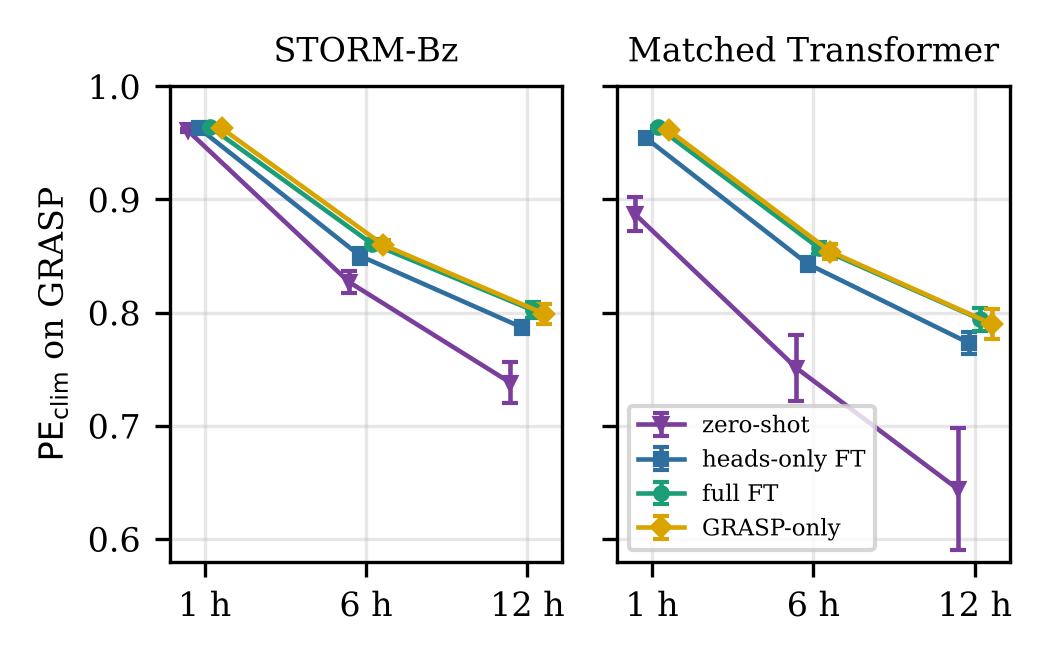
\includegraphics[width=0.92\columnwidth]{figures/fig_grasp_transfer.png}
\caption{GRASP skill by regime (mean \(\pm\) standard deviation over seeds,
averaged over folds). Zero-shot (purple) shows the largest difference between models.}
\label{fig:grasp}
\end{figure}

%% ====================================================================
\section{Discussion and Limitations}
\label{sec:limits}
%% ====================================================================
Our absolute skill is in the range of recent hourly studies (e.g.\
0.940/0.828/0.747 at 1/6/12\,h in~\cite{sun2024}), but cadence, satellite,
energy channel and test period differ, so these numbers are not a ranking.
Within our protocol the main lesson is that the simplest effective idea, a
residual over persistence, is what makes a Transformer useful at short lead,
and that physics-motivated modules should be judged by robustness as well as by
clean accuracy. Our earlier, leakier pipeline reported 12\,h PE 0.854 on the same 2018--20
period as block A, against 0.804 here, which illustrates how strongly evaluation choices affect
reported skill.

\textbf{Operational reading.} For a GEO operator the results suggest a
simple recipe: anchor every horizon on persistence, rely on solar-wind drivers
for 6--12\,h warnings, and prefer the gated model where driver data are noisy or
missing, or when a new sensor has little history, since it degrades gracefully
in both cases. When several months of target data exist, fine-tuning or even
target-only training is sufficient.

\textbf{Limitations.} (1) The input Kp and Dst are definitive values; real-time
products differ, and solar-wind drivers are not forecast, so 12\,h forecasts
assume upstream data only up to the forecast time. (2) Blocks B and C train on
data from both sides of the test period. (3) Only 937 test windows are storm
time and the case study is a single event. (4) GRASP covers 14 months near
solar minimum, is uncalibrated against GOES and was run without driver inputs;
the residual-head control was not run on GRASP, so its zero-shot advantage
cannot be attributed to the delay and gate rather than the residual. (5) Tests
are uncorrected for multiplicity and seeds measure initialisation variance on
fixed splits.

%% ====================================================================
\section{Conclusion}
%% ====================================================================
Under a leakage-free, multi-period, multi-seed protocol, STORM-PhysNet gives
the best 1\,h forecasts of GEO \({>}2\)\,MeV flux in every test block and
skill far above persistence at 6--12\,h, although a simpler residual
Transformer is slightly better at those horizons. Its delay and gate do not add
clean-data accuracy but coincide with large gains in robustness to corrupted
drivers and in zero-shot transfer to the GSAT-19 GRASP sensor, where fine-tuning
and target-only training then reach the same skill. We release the protocol,
code and all predictions so that future models for Indian-longitude GEO assets
can be compared on equal terms.

\section*{Data Availability}
Code, configurations, the leakage-free data pipeline, per-run predictions,
tables and figures are available at
\url{https://github.com/bnsama29-cloud/STORM-PhysNet-L1}. GOES-15 data are
from NOAA NCEI (\url{https://www.ngdc.noaa.gov/stp/satellite/goes/}), OMNI from
NASA OMNIWeb (\url{https://omniweb.gsfc.nasa.gov/}) and GSAT-19 GRASP from ISSDC
(\url{https://pradan1.issdc.gov.in/grasp/}).

\section*{Acknowledgment}
The authors thank the GOES, OMNI and GRASP data providers.

\FloatBarrier
\begin{thebibliography}{99}
\footnotesize
\bibitem{baker2018}
D.~N. Baker, P.~J. Erickson, J.~F. Fennell, J.~C. Foster, A.~N. Jaynes, and
P.~T. Verronen, ``Space weather effects in the Earth's radiation belts,''
\emph{Space Sci. Rev.}, vol.~214, no.~1, Art.~no.~17, 2018,
doi:10.1007/s11214-017-0452-7.
\bibitem{horne2005}
R.~B. Horne \emph{et al.}, ``Wave acceleration of electrons in the Van Allen
radiation belts,'' \emph{Nature}, vol.~437, pp.~227--230, 2005,
doi:10.1038/nature04033.
\bibitem{baker1990}
D.~N. Baker, R.~L. McPherron, T.~E. Cayton, and R.~W. Klebesadel, ``Linear
prediction filter analysis of relativistic electron properties at
6.6\,\(R_E\),'' \emph{J. Geophys. Res.}, vol.~95, no.~A9, pp.~15133--15140,
1990, doi:10.1029/JA095iA09p15133.
\bibitem{perry2010}
K.~L. Perry, G.~P. Ginet, A.~G. Ling, and R.~V. Hilmer, ``Comparing
geosynchronous relativistic electron prediction models,'' \emph{Space
Weather}, vol.~8, Art.~no.~S12002, 2010, doi:10.1029/2010SW000581.
\bibitem{wei2018}
L.~Wei, Q.~Zhong, R.~Lin, J.~Wang, S.~Liu, and Y.~Cao, ``Quantitative
prediction of high-energy electron integral flux at geostationary orbit based
on deep learning,'' \emph{Space Weather}, vol.~16, no.~7, pp.~903--916, 2018,
doi:10.1029/2018SW001829.
\bibitem{son2022}
J.~Son, Y.-J. Moon, and S.~Shin, ``72-hour time series forecasting of hourly
relativistic electron fluxes at geostationary orbit by deep learning,''
\emph{Space Weather}, vol.~20, no.~10, Art.~no.~e2022SW003153, 2022,
doi:10.1029/2022SW003153.
\bibitem{tan2024}
M.~Tan, X.~Si, S.~Teng, X.~Wu, and X.~Tao, ``Comparative analysis of TPA-LSTM
and Transformer models for forecasting GEO radiation belt electron fluxes,''
\emph{Space Weather}, vol.~22, no.~11, Art.~no.~e2024SW004119, 2024,
doi:10.1029/2024SW004119.
\bibitem{sun2024}
X.~Sun \emph{et al.}, ``A modeling study of \({\geq}2\)\,MeV electron fluxes in
GEO at different prediction time scales based on LSTM and transformer
networks,'' \emph{J. Space Weather Space Clim.}, vol.~14, Art.~no.~25, 2024,
doi:10.1051/swsc/2024021.
\bibitem{sun2025}
X.~Sun \emph{et al.}, ``Enhancing \({\geq}2\)\,MeV electron fluence predictions
in GEO orbit through three deep learning strategies,'' \emph{Space Weather},
vol.~23, no.~8, Art.~no.~e2025SW004519, 2025, doi:10.1029/2025SW004519.
\bibitem{camporeale2019}
E.~Camporeale, ``The challenge of machine learning in space weather:
Nowcasting and forecasting,'' \emph{Space Weather}, vol.~17, no.~8,
pp.~1166--1207, 2019, doi:10.1029/2018SW002061.
\bibitem{kapoor2023}
S.~Kapoor and A.~Narayanan, ``Leakage and the reproducibility crisis in
machine-learning-based science,'' \emph{Patterns}, vol.~4, no.~9,
Art.~no.~100804, 2023, doi:10.1016/j.patter.2023.100804.
\bibitem{zeng2023}
A.~Zeng, M.~Chen, L.~Zhang, and Q.~Xu, ``Are Transformers effective for time
series forecasting?'' in \emph{Proc. AAAI Conf. Artif. Intell.}, vol.~37,
no.~9, 2023, pp.~11121--11128, doi:10.1609/aaai.v37i9.26317.
\bibitem{zhao2025}
Y.~Zhao \emph{et al.}, ``Cross-calibrated FY-4A and GOES-15 data for
\({>}2\)\,MeV electron flux prediction at geosynchronous orbit: A machine
learning approach,'' \emph{Space Weather}, vol.~23, no.~11,
Art.~no.~e2025SW004419, 2025, doi:10.1029/2025SW004419.
\bibitem{forsyth2020}
C.~Forsyth, C.~E.~J. Watt, M.~K. Mooney, I.~J. Rae, S.~D. Walton, and
R.~B. Horne, ``Forecasting GOES 15 \({>}2\)\,MeV electron fluxes from solar
wind data and geomagnetic indices,'' \emph{Space Weather}, vol.~18, no.~8,
Art.~no.~e2019SW002416, 2020, doi:10.1029/2019SW002416.
\bibitem{lim2021}
B.~Lim, S.~\"O. Ar{\i}k, N.~Loeff, and T.~Pfister, ``Temporal Fusion
Transformers for interpretable multi-horizon time series forecasting,''
\emph{Int. J. Forecast.}, vol.~37, no.~4, pp.~1748--1764, 2021,
doi:10.1016/j.ijforecast.2021.03.012.
\bibitem{morley2018}
S.~K. Morley, T.~V. Brito, and D.~T. Welling, ``Measures of model performance
based on the log accuracy ratio,'' \emph{Space Weather}, vol.~16, no.~1,
pp.~69--88, 2018, doi:10.1002/2017SW001669.
\bibitem{bergmeir2018}
C.~Bergmeir, R.~J. Hyndman, and B.~Koo, ``A note on the validity of
cross-validation for evaluating autoregressive time series prediction,''
\emph{Comput. Stat. Data Anal.}, vol.~120, pp.~70--83, 2018,
doi:10.1016/j.csda.2017.11.003.
\bibitem{king2005}
J.~H. King and N.~E. Papitashvili, ``Solar wind spatial scales in and
comparisons of hourly Wind and ACE plasma and magnetic field data,''
\emph{J. Geophys. Res.}, vol.~110, Art.~no.~A02104, 2005,
doi:10.1029/2004JA010649.
\bibitem{vaswani2017}
A.~Vaswani \emph{et al.}, ``Attention is all you need,'' in \emph{Proc. Adv.
Neural Inf. Process. Syst.}, 2017, pp.~5998--6008.
\bibitem{seitzer2022}
M.~Seitzer, A.~Tavakoli, D.~Antic, and G.~Martius, ``On the pitfalls of
heteroscedastic uncertainty estimation with probabilistic neural networks,''
in \emph{Proc. Int. Conf. Learn. Represent. (ICLR)}, 2022.
\end{thebibliography}

\end{document}
